\section{Gradient Boosted Decision Trees}
\begin{multicols}{2}

Another tree based ensemble method that's gain wide use in real world application is gradient boosted decision trees~--- GBDT. 

Like random forest, gradient boosted trees used an ensemble of multiple tress to create more powerful prediction models for classification and regression. 

In this lecture, we'll provide a brief overview of gradient boosted decision trees, along with the discussion of their key parameters, the control model complexity. 

Unlike the random forest method that builds and combines a forest of randomly different trees in parallel, the key idea of gradient boosted decision trees is that they build a \emph{series} of trees. Where each tree is trained, so that it attempts to correct the mistakes of the previous tree in the series. 

\begin{center}
	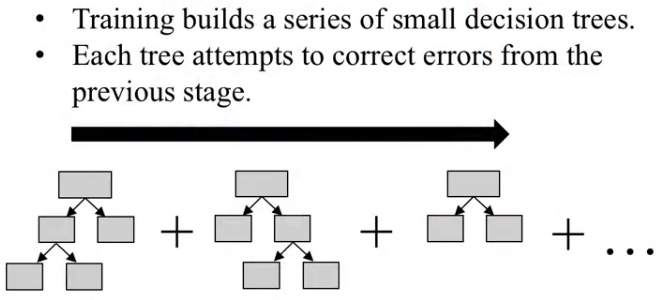
\includegraphics[width=\linewidth]{img/GBDT-1.png} 
\end{center}

Typically, gradient boosted tree ensembles use lots of shallow trees known in machine learning as \emph{weak learners}. Built in a \emph{non-random} way, to create a model that makes fewer and fewer mistakes as more trees are added.  

Once the model is built, making predictions with a gradient boosted tree models is fast and doesn't use a lot of memory. 

\begin{center}
	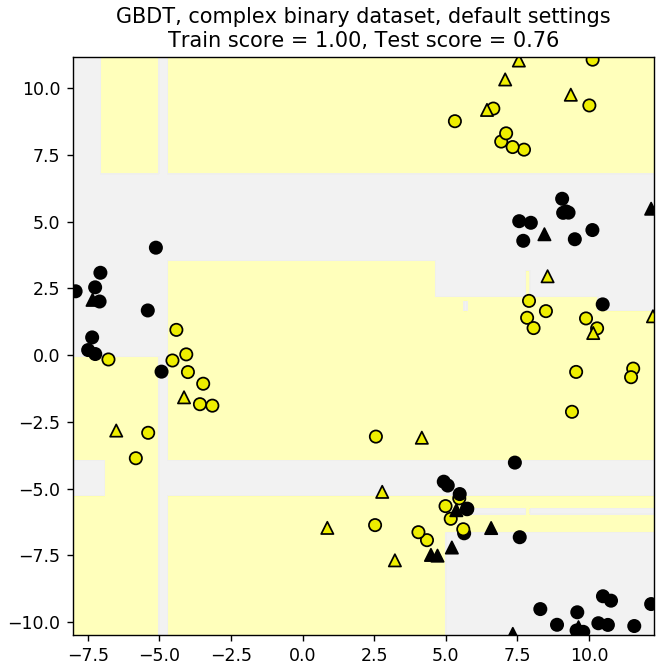
\includegraphics[width=\linewidth]{img/GBDT-3.png} 
\end{center}


Like random forests, the \texttt{number of estimators} in the gradient boosted tree ensemble is an important parameter in controlling model complexity. 

A new parameter that does not occur with random forest is something called the \texttt{learning_rate}. The learning rate controls how the gradient boost the tree algorithms builds a series of collective trees. When the learning rate is \emph{high}, each successive tree puts strong emphases on correcting the mistakes of its predecessor, and thus may result in a more complex individual tree, and those overall are more complex model. With \emph{smaller} settings of the learning rate, there's less emphasis on thoroughly correcting the errors of the previous step, which tends to lead to simpler trees at each step. 

{\scriptsize
\begin{verbatim}
from sklearn.ensemble import GradientBoostingClassifier
from sklearn.model_selection import train_test_split

X_train, X_test, y_train, y_test = 
    train_test_split(X_D2, y_D2, random_state = 0)

clf = GradientBoostingClassifier().fit(X_train, y_train)
...
GBDT, Fruit dataset, default settings
Accuracy of GBDT classifier on training set: 1.00
Accuracy of GBDT classifier on test set: 0.80
\end{verbatim}
}


\begin{center}
	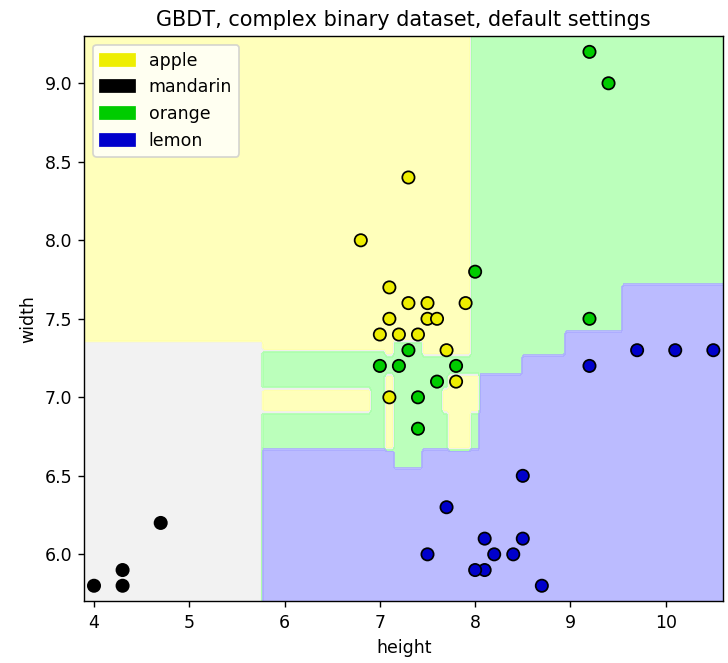
\includegraphics[width=\linewidth]{img/GBDT-4.png} 
\end{center}

Here's an example showing how to use gradient boosted trees in scikit-learn on our sample fruit classification test, plotting the decision regions that result. The code is more or less the same as what we used for random forests. 

But from the sklearn.ensemble module, we import the \texttt{GradientBoostingClassifier} class. We then create the \texttt{GradientBoostingClassifier} object, and fit it to the training data in the usual way. By default, the \texttt{learning rate} parameter is set to \textbf{0.1}, the \texttt{n_estimators} parameter giving the number of trees to use is set to \textbf{100}, and the \textbf{max_depth} is set to \textbf{3}. As with random forests, you can see the decision boundaries have that box-like shape that's characteristic of decision trees or ensembles of trees. 

Now let's apply gradient boosted decision trees to the breast cancer dataset. This code trains two different gradient boosted classifiers. The first one uses the default settings. 

{\scriptsize
\begin{verbatim}
Breast cancer dataset (learning_rate=0.1, max_depth=3)
Accuracy of GBDT classifier on training set: 1.00
Accuracy of GBDT classifier on test set: 0.96

Breast cancer dataset (learning_rate=0.01, max_depth=2)
Accuracy of GBDT classifier on training set: 0.97
Accuracy of GBDT classifier on test set: 0.97
\end{verbatim}
}

We can see that the first result has perfect accuracy on the training set, which indicates the model is likely overfitting. 

Two ways to learn a less complex gradient boosted tree model are, to reduce the \texttt{learning_rate}, so that each tree doesn't try as hard to learn a more complex model, that fixes the mistakes of its predecessor. And to reduce the \texttt{max_depth} parameter for the individual trees in the ensemble. 

The second classifier example makes these changes in the parameters. And you can see, that the training set accuracy does decrease, while the test set accuracy increases slightly. 

\subsection{Pros and Cons}

Gradient boosted decision trees are among the best off-the-shelf supervised learning methods available. Achieving excellent accuracy with only modest memory and runtime requirements to perform prediction, once the model has been trained. 

Some major commercial applications of machine learning have been based on gradient boosted decision trees. 

Like other decision tree based learning methods, you don't need to apply feature scaling for the algorithm to do well. And the futures can be a mix of binary, categorical and continuous types. 

Boosted decision trees do have several downsides. So like random forests, ensembles of trees are very difficult for people to interpret, compared to individual decision trees. However, this often may not matter for many applications where prediction accuracy is the most important goal. 

Gradient boosted methods can require careful tuning of the learning rate and other parameters. And the training process can require a lot of computation. 

And like the other tree based methods we saw, using gradient boosted methods for text classification or other scenarios. Where the featured space has thousands of features with sparse values, is usually not a good choice for accuracy and computational cost reasons. 

\subsection{Key Parameters}

The key parameters controlling model complexity for gradient boosted tree models are, \texttt{n_estimators} which sets the number of small decisions trees the week learns to use in the ensemble, and the \texttt{learning_rate}. 

Typically, these two parameters are tuned together. Since making the learning rates smaller, will require more trees to maintain model complexity. 

Unlike random forest, increasing an \texttt{n_estimators} can lead to overfeeding. So typically, the \texttt{n_estimators} setting is chosen to best exploit the speed and memory capabilities of the system during the training. And other parameters like the \texttt{learning_rate} are then adjusted, given that fixed an n_estimators setting. 

The \texttt{max_depth} parameter can also have an effect of model complexity, but controlling the depth, and has a complexity of the individual trees. The gradient boosting method assumes, that each trees is a weak learner, and so the \texttt{max_depth} parameter is usually quite small, on the order of three to five, for most applications. 

\end{multicols}